% ---------
% --------
%!TEX TS-program = pdflatex
%!TEX encoding = UTF-8 Unicode
%!TEX spellcheck = English (Aspell)

\documentclass[11pt]{article}
\usepackage{lucy,handout,graphicx}
\usepackage{fourier-orns}
\usepackage{mathtools}
\usepackage[normalem]{ulem} % either use this (simple) or
\usepackage{tikz}
\usetikzlibrary{graphs}

\allowdisplaybreaks


\begin{document}

\noindent Name \underline{\hspace{12cm}}\\

\begin{center}
\Large\textbf{CSCI 332, Fall 2026}\\
\LARGE\textbf{Exam 1 Practice 1}
\end{center}

\noindent This exam consists of the following sections:
\begin{enumerate}
    \item Stable Matching
    \item Algorithm Analysis
    \item Recursion
    \item 1D Dynamic Programming
\end{enumerate}

You may use a double sided 3x5 handwritten notecard of notes during the test but no other resources.

For BUBBLE SHEET sub sections, fill in your answers on the provided bubble sheet. Some questions may have
multiple correct answers; be sure to select all that apply.

For HANDWRITTEN subsections, write your answers on the exam paper.

Good luck!

\newpage

\begin{center}
\LARGE\textbf{Section 1 (Stable Matching)\\}%
\end{center}
\subsection*{Bubble sheet}


\begin{enumerate}

\item Is $\{(h_1, s_4), (h_2, s_1), (h_3, s_3), (h_4, s_2)\}$ a stable matching for the given preference lists?

\begin{table}[h]
\centering
\begin{tabular}{c | l || c | l}
\textbf{Hospital} & \textbf{Preferences} & \textbf{Student} & \textbf{Preferences} \\
\hline
$h_1$ & $s_2 , s_3 , s_4 , s_1$ & $s_1$ & $h_3 , h_1 , h_2 , h_4$ \\
$h_2$ & $s_1 , s_3 , s_2 , s_4$ & $s_2$ & $h_2 , h_3 , h_4 , h_1$ \\
$h_3$ & $s_3 , s_4 , s_2 , s_1$ & $s_3$ & $h_3 , h_2 , h_4 , h_1$ \\
$h_4$ & $s_1 , s_3 , s_2 , s_4$ & $s_4$ & $h_4 , h_1 , h_3 , h_2$ \\
\end{tabular}
\end{table}

Select A for yes and B for no.

\item Given the matching
$\{(h_4, s_1), (h_1, s_3), (h_3, s_4), (h_2, s_2)\}$ and the
preference lists below,
select all unstable pairs from the list.

\begin{table}[h]
\centering
\begin{tabular}{c | l || c | l}
\textbf{Hospital} & \textbf{Preferences} & \textbf{Student} & \textbf{Preferences} \\
\hline
$h_1$ & $s_1 , s_2 , s_3 , s_4$ & $s_1$ & $h_3 , h_2 , h_1 , h_4$ \\
$h_2$ & $s_1 , s_2 , s_4 , s_3$ & $s_2$ & $h_1 , h_2 , h_3 , h_4$ \\
$h_3$ & $s_2 , s_1 , s_3 , s_4$ & $s_3$ & $h_1 , h_3 , h_4 , h_2$ \\
$h_4$ & $s_4 , s_2 , s_3 , s_1$ & $s_4$ & $h_3 , h_4 , h_2 , h_1$ \\
\end{tabular}
\end{table}

\begin{enumerate}[A.]
    \item $(h_4, s_1)$
    \item $(h_2, s_4)$
    \item $(h_2, s_1)$
    \item $(h_3, s_3)$
    \item $(h_1, s_2)$
\end{enumerate}


The following questions refer to the Gale-Shapley algorithm for
stable matching.

    \begin{algo}
    Gale-Shapley(preference lists for $n$ hospitals and $n$ students)\+\\
    Let $M$ be an empty matching\\
    While some hospital $h$ is umatched and hasn't proposed to every student:\+ \\
        Let $s$ be the first student on $h$'s list to whom $h$ has not yet proposed\\
        If $s$ is unmatched:\+\\
            Add $(h,s)$ to $M$\-\\
        Else $s$ is matched to $h'$:\+\\
            If $s$ prefers $h$ to $h'$:\+\\
                Remove $(h',s)$ from $M$\\
                Add $(h,s)$ to $M$\-\\
            Else $s$ prefers $h'$ to $h$:\+\\
                Do nothing\-\-\-\\
    Return $M$\\
    \end{algo}

\item Does the Gale-Shapley algorithm always terminate with a stable matching?
Select A for yes and B for no.

\item Are there inputs for which the Gale-Shapley algorithm runs in $\Theta(n)$ time?
Select A for yes and B for no.

\item Are there inputs for which the Gale-Shapley algorithm runs in $\Theta(n^2)$ time?
Select A for yes and B for no.

\item Are there inputs for which the Gale-Shapley algorithm runs in $\Theta(n^3)$ time?
Select A for yes and B for no.

\item What is the stable matching returned by the Gale-Shapley algorithm on the
following preference list?

\begin{table}[h]
\centering
\begin{tabular}{c | l || c | l}
\textbf{Hospital} & \textbf{Preferences} & \textbf{Student} & \textbf{Preferences} \\
\hline
$h_1$ & $s_1 , s_2 , s_3 , s_4$ & $s_1$ & $h_3 , h_2 , h_1 , h_4$ \\
$h_2$ & $s_1 , s_2 , s_4 , s_3$ & $s_2$ & $h_1 , h_2 , h_3 , h_4$ \\
$h_3$ & $s_2 , s_1 , s_3 , s_4$ & $s_3$ & $h_1 , h_3 , h_4 , h_2$ \\
$h_4$ & $s_4 , s_2 , s_3 , s_1$ & $s_4$ & $h_3 , h_4 , h_2 , h_1$ \\
\end{tabular}
\end{table}

\begin{enumerate}[A.]
    \item $\{(h_1, s_1), (h_2, s_1), (h_3, s_2), (h_4, s_4)\}$
    \item $\{(h_1, s_1), (h_2, s_2), (h_3, s_3), (h_4, s_4)\}$
    \item $\{(h_1, s_4), (h_2, s_3), (h_3, s_1), (h_4, s_2)\}$
    \item $\{(h_1, s_2), (h_2, s_3), (h_3, s_1), (h_4, s_4)\}$
    \item $\{(h_1, s_3), (h_2, s_1), (h_3, s_4), (h_4, s_2)\}$
\end{enumerate}


\item (5 points) True or false? In every instance of the
 Stable Matching Problem, there is a stable matching containing a pair $(m,w)$
 such that $m$ is ranked first on the preference list of $w$ and $w$ is ranked
 first on the preference list of $m$. Select A for true and B for false.

\newpage


\begin{center}
\LARGE\textbf{Section 2 (Algorithm Analysis)\\}%
\end{center}

\subsection*{Bubble sheet}

\item Recall that the definition of big O is as follows:
\emph{$f(n)$ is $O(g(n))$ if there exist positive constants $c$ and $n_0$ such
that for all $n >= n_0$, $f(n) \leq c \cdot g(n)$.} Which $n_0$ and $c$ can be
used to show that $9n^2 + n + 10$ is $O(n^3)$?
\begin{enumerate}[A.]
    \item $n_0 = 1$, $c = 4$
    \item $n_0 = 1$, $c = 10$
    \item $n_0 = 1$, $c = 1000$
    \item $n_0=10, c = 4$
    \item $n_0 = 100$, $c = 1$

\end{enumerate}

\item Select all of the true statements below.
\begin{enumerate}[A.]
    \item $\log(100 \cdot n^{5n})$ is $\Theta(n \log n)$
    \item $\log(100 \cdot n^{5n})$ is $\Theta(n^n)$
    \item $\log(100 \cdot n^{5n})$ is $\Theta(5^n)$
    \item $\log(100 \cdot n^{5n})$ is $\Theta(n^n \log n)$
    \item $\log(100 \cdot n^{5n})$ is $\Theta(n^5 \log 100)$
\end{enumerate}

\item Select all the functions that are $O(n^2)$.
\begin{enumerate}[A.]
    \item $5n^2 + 3n + 20$
    \item $n \log n$
    \item $n^2 + n \log n$
    \item $0.5 n^2 - 10 n + 2000$
    \item $n^3$

\end{enumerate}

\item Select all functions that are $\Omega(n^2)$.

\begin{enumerate}[A.]
    \item $5n^2 + 3n + 20$
    \item $n \log n$
    \item $n^2 + n \log n$
    \item $0.5 n^2 - 10 n + 2000$
    \item $n^3$

\end{enumerate}

\item Select all functions that are $\Theta(n^2)$.

\begin{enumerate}[A.]
    \item $5n^2 + 3n + 20$
    \item $n \log n$
    \item $n^2 + n \log n$
    \item $0.5 n^2 - 10 n + 2000$
    \item $n^3$

\end{enumerate}

\item Select all functions $f(n)$ such that the worst-case runtime of
Algorithm-1 below is $\Theta(f(n))$.

    \begin{algo}
    Algorithm-1(array $A$ of length $n$):\+\\
    Result = 0\\
    For each $i$ in $1$ to $n$:\+\\
    For each $j$ in $1$ to $i$:\+\\
    Set Result to $A[j]$ times Result\-\- \\
    Return Result\\
    \end{algo} 

\begin{enumerate}[A.]
    \item $n$
    \item $\log n$
    \item $n^2$
    \item $n^3$
    \item $n!$
\end{enumerate}



\subsection*{Handwritten}
\item (10 points)
You suspect that in the most recent update to your favorite software package,
the implementation of your favorite function \texttt{do-stuff} was replaced by a $\Theta(n^2)$ 
algorithm, whereas it was a $\Theta(n^3)$ algorithm before. Whatever the runtime is, you know that
it is the same for all input classes (that is, the worst case and best case runtimes are equal).
Unfortunately, the package is
closed-source and you cannot inspect the source code; you can only run the function on
various-sized inputs and record its runtime on those inputs.

Describe an experiment that you could run to verify your hunch. That is, tell us what kinds
of input sizes you will run \texttt{do-stuff} on and how you will use their runtimes to
determine whether the algorithm is $\Theta(n^2)$ or $\Theta(n^3)$.

\item (10 points) Consider the following algorithm to determine whether a number can be written
as the sum of two perfect squares. For example, $40=4+36=2^2+6^2$, so SumOfSquares($40$) returns
true, whereas SumOfSquares($42$) returns false, because there are no integers $a,b$ so that
$42=a^2 + b^2$.

    \begin{algo}
    \underline{SumOfSquares(n):}\+\\
    $a = 0$\\
    $b = \floor{\sqrt{n}}$\\
    while $a <= b$:\+\\
        $s = a^2 + b^2$\\
        if $s == n$:\+\\
            return true\-\\
        if $s < n$:\+\\
            $a = a + 1$\-\\
        else:\+\\
            $b = b - 1$\-\-\\
    return false\\
    \end{algo}

    \begin{enumerate}
        \item Describe the class of best-case inputs and give the simplest $f(n)$ so that
        their runtime is $\Theta(f(n))$.
        \item Describe the class of worst-case inputs and give the simplest $f(n)$ so that
        their runtime is $\Theta(f(n))$.
    \end{enumerate}


\newpage

\begin{center}
\LARGE\textbf{Section 3 (Recursion)\\}%
\end{center}

% Source: cs332-fall2025/exams/exam2/main.tex
\subsection*{Handwritten}
\item (10 points) Given the following (meaningless) divide and conquer algorithm,
what is the recurrence relation that describes its running time?

    \begin{algo}
    wut(integer array $A$ of length $n$): \+ \\
    if $n \leq 1$:\+\\
        return $A$\-\\
    else:\+\\
    Let $A_1, A_2, A_3$ be the first third, middle third, and last third of $A$\\
    $X_1$ = wut($A_1$)\\
    $X_2$ = wut($A_2$)\\
    $X_3$ = wut($A_3$)\\
    let array $C$ be a new array of length $n$\\
    for $i$ from 1 to $n$:\+\\
        for $j$ from 1 to $n$:\+\\
            $C[i \% j] = \textrm{first element of } X_1 + \textrm{middle element of
            }X_2 +\textrm{last element of } X_3$\-\-\\
    return $C$\-\\
    \end{algo}

$T(1) =$ \underline{\hspace{2cm}}\\

$\begin{array}{lccc}
T(n) = & \underline{\hspace{5cm}} & + & \underline{\hspace{5cm}} \\[2pt]
& \text{work done by recursive calls} & &  \text{nonrecursive work}
\end{array}$

\item (15 points)

Consider the recurrence $T(n) = 4T(n/3) + n, T(1) = 1$.

\begin{enumerate}[(a)]

\item (5 points) In the left boxes, draw the first three levels of this recursion tree.
In the boxes next to them, write the total work on that level.

\begin{center}
\begin{tikzpicture}[
  boxL/.style={draw, rectangle, minimum width=9cm, minimum height=2.2cm, inner sep=6mm},
  boxR/.style={draw, rectangle, minimum width=4.1cm, minimum height=2.2cm, inner sep=6mm},
  smalllabel/.style={font=\scriptsize, anchor=north west}
]

\node[boxL] (L0) at (0,4.0) {};
\node[smalllabel] at (L0.north west) {Level 0};

\node[boxL] (L1) at (0,1.5) {};
\node[smalllabel] at (L1.north west) {Level 1};

\node[boxL] (L2) at (0,-1) {};
\node[smalllabel] at (L2.north west) {Level 2};

\node[boxR] (R0) at (7,4.0) {};
\node[smalllabel] at (R0.north west) {Sum level 0};

\node[boxR] (R1) at (7,1.5) {};
\node[smalllabel] at (R1.north west) {Sum level 1};

\node[boxR] (R2) at (7,-1) {};
\node[smalllabel] at (R2.north west) {Sum level 2};

\end{tikzpicture}
\end{center}
\item (3 points) What is the work per level in terms of level $\ell$?
\vspace{1in}
\item (2 points) Is the work per level (circle one)
\begin{itemize}
    \item increasing (work is dominated by leaves)
    \item decreasing (work is dominated by root)
    \item the same (work is the same at every level)
\end{itemize}
\item (3 points)  What is the total number of levels in the tree? (fill in the base and the argument of the logarithm)
\[
\text{number of levels} = \log_{\underline{\hspace{1cm}}}(\underline{\hspace{1cm}})
\]

\item (2 points) What is the overall non-recursive runtime of the recurrence?

\vspace{1in}
\end{enumerate}

\item (10 points total) In this problem you will write a \textbf{divide and conquer} algorithm for the following problem: you
are given an array $A$ of $n$ integers (which may be positive, negative, or zero).
You know that the array is \emph{unimodal}, meaning that there is an index $i^*$ such that
$A[1] < A[2] < \cdots < A[i^*]$ and $A[i^*] > A[i^* + 1] > \cdots > A[n]$.
Your task is to find the index $i^*$ (the index of the maximum element) in $O(\log n)$ time.
Assume that the indices start at 1.

For example, if $A = [-1, 3, 3, 5, 8, 12, 4, 2]$, then the output should be $6$ since
$A[6] = 12$ is the maximum element.

\begin{enumerate}

    \item (2 points) In order to achieve an $O(\log n)$ runtime, you can only make one recursive
    call per level of recursion, and it must take only constant time. You decide that you will divide
    the array in half at each step. How will you decide which half on which to make your next recursive call?
    \vspace{2in}

    \item (6 points) Write a \textbf{recursive} algorithm to find $i^*$ that runs in $O(\log n)$ time.

    \begin{algo}
    Max(unimodal array $A$ of length $n$):\+\\
    \\
    \\
    \\
    \\
    \\
    \\
    \\
    \\
    \\
    \\
    \\
    \\
    \\
    \\
    \\
    \\
    \\
    \\
    \\
    \\
    \\
    \\
    \\
    \\
    \\
    \\
    \\
    \\
    \\
    \\
    \hspace{5in}

    \end{algo}
\end{enumerate}


\newpage

\begin{center}
\LARGE\textbf{Section 4 (1D Dynamic Programming)\\}%
\end{center}

\subsection*{Handwritten}
\item (10 points) Given the following (meaningless) recursive definition of a subproblem, draw the 
recursion tree for a call to $huh(5)$ with each node labeled with the value of the argument to $huh$.

\begin{equation*}
    huh(i) =
    \begin{cases}
        4 & if i = 1 \\
        -100 & if i = 2\\
        0 & if i = 3\\
        \min \left(2 + huh(i-1), huh(i-3)\right) & if i > 3 \\

    \end{cases}
\end{equation*}

The first node is provided for you.

\begin{center}
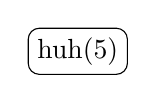
\begin{tikzpicture}
  \node[rectangle, draw, rounded corners] {huh(5)};
\end{tikzpicture}
\end{center}
\vspace{2in}


    \item (10 points)
    In this problem, you will need to write the formal recursive definition
    for the subproblem (step two of our four steps for writing dynamic programming algorithms)
    for the following problem.
    
    \textbf{The problem.} In your country, there are only coins of denominations
    1, 3, and 4. Given a pasitive integer n, what is the fewest number of
    coins you can use to represent n?

    To solve this problem, we first write the English definition of the subproblem.

    \textbf{1. The subproblem.} Let $MinCoins(i)$ be the minimum number of coins needed to represent the amount $i$.

    Next, we think about the recursive relationship between subproblems. You notice that in order to make $i$,
    you could either have made $i-1$ and added a 1-coin, or made $i-3$ and added a 3-coin,
    or made $i-4$ and added a 4-coin. Using this observation, fill in the formal recursive
    definition for $MinCoins(i)$ below.

    \textbf{2. The recursive definition.} The recursive relationship can be expressed as:
    (fill in both recursive case(s) and base case(s). You may not need every line provided!)

    \begin{equation*}
        MinCoins(i) =
        \begin{cases}
        \underline{\hspace{3in}} & if i \underline{\hspace{1in}} \\
        \underline{\hspace{3in}} & if i \underline{\hspace{1in}} \\
        \underline{\hspace{3in}} & if i \underline{\hspace{1in}} \\
        \underline{\hspace{3in}} & if i \underline{\hspace{1in}} \\
        \underline{\hspace{3in}} & if i \underline{\hspace{1in}} \\
        \end{cases}
    \end{equation*}

    \item (10 points) In this problem, you will need to write algorithm pseudocode  
    (step four of our four steps for writing dynamic programming algorithms)
    for the following problem.

\textbf{The problem.} You are given a rod of length $n$ and a price list
$p_1, p_2, \ldots, p_n$, where $p_i$ is the price of a rod piece of length $i$.
You may cut the rod into any number of integer-length pieces, or leave it
uncut. Each piece of length $i$ sells for $p_i$, and making cuts has no cost.
Describe an algorithm to determine the maximum revenue obtainable from the rod.

To solve this problem, we first write the English definition of the subproblems.

    \textbf{1. The subproblem.} Let $MaxRevenue(i)$ be the maximum revenue obtainable
    from a rod of length $i$.

    Next, we think about the recursive relationship between subproblems. For a rod
    of length $i$, the first piece can have any length $j$ from $1$ to $i$. Selling
    that piece earns $p_j$, and the remaining rod has length $i-j$. Using this
    observation, write the formal recursive definition for $MaxRevenue(i)$ below.

    \textbf{2. The recursive definition.} 

    \begin{equation*}
        MaxRevenue(i) =
        \begin{cases}
            0 & if i = 0 \\
            \max_{1 \leq j \leq i} (p_j + MaxRevenue(i-j)) & if i > 0
        \end{cases}
    \end{equation*}

    \textbf{3. How to memoize.} We can use an array of length $n+1$ to store the
    values of $MaxRevenue(i)$ for $0 \leq i \leq n$ and fill it in increasing order.


    \textbf{4. Write the algorithm.} Using the above information, finish the pseudocode
    to find the maximum revenue obtainable from a rod of length $n$, given the
    price list $p[1..n]$.
    \begin{algo}
    RodCutting($p[1..n], n$):\+\\
    Let array $R$ be an array of length $n+1$\\
    \# what is the base case?\\
    \\
    \\
    \\
    \\
    \\
    \# how should we fill in the rest of the array?\\
    \\
    \\
    \\
    \\
    \\
    \\
    \\
    \\
    \# what should we return to get the final answer?\\
    \\
    \\
    \\
    \hspace{5in}
    \end{algo}




\end{enumerate}
\end{document}
